\documentclass[a4paper,12pt,reqno, english]{amsart}  
\usepackage[utf8]{inputenc}
\usepackage[T1]{fontenc}
\usepackage{amsmath}
\usepackage[margin=1in]{geometry}


\usepackage{amsthm}

\usepackage{framed}

\usepackage{amssymb}
\usepackage{tikz}
\usepackage{enumerate}
\usepackage[mathscr]{euscript}

\newcommand{\pd}[2]{\frac{\partial #1}{\partial #2}}
\newcommand{\ee}[1]{\times 10^{#1}}
\newcommand{\td}{\textbf{TO DO!!!!!!!}}
\newcommand{\Span}[1]{\mathrm{Span} ( #1 )}
\newcommand{\inv}{^{-1}}
\newcommand{\dgh}{d_{\mathrm{GH}}}
\newcommand{\dB}{d_{\mathrm{B}}}
\newcommand{\dH}{d_{\mathrm{H}}}
\newcommand{\cset}{\mathrm{K}}
\newcommand{\dgm}{\mathrm{dgm}}
\newcommand{\pow}{\mathrm{pow}}
\newcommand{\diam}{\mathrm{diam}}
\newcommand{\ecc}{\mathrm{ecc}}
\newcommand{\dis}{\mathrm{dis}}
\newcommand{\ud}{\mathrm{u}}




\newcommand{\geng}[1]{\langle #1 \rangle}
\newcommand{\set}[1]{\{ #1\}}
\newcommand{\id}{\text{id}}
\DeclareMathOperator{\terior}{int}
\DeclareMathOperator{\rank}{rank}
\DeclareMathOperator{\Hom}{Hom}
\DeclareMathOperator{\Tor}{Tor}
\DeclareMathOperator{\Ext}{Ext}
\DeclareMathOperator{\Gal}{Gal}
\DeclareMathOperator{\Tr}{Tr}
\DeclareMathOperator{\Aut}{Aut}
\DeclareMathOperator{\coker}{coker}
\DeclareMathOperator{\im}{im}
\DeclareMathOperator{\ult}{ult}
\DeclareMathOperator{\hyp}{hyp}
\newcommand{\Z}{\mathbb{Z}}
\newcommand{\R}{\mathbb{R}}
\newcommand{\Q}{\mathbb{Q}}
\newcommand{\C}{\mathbb{C}}
\newcommand{\N}{\mathbb{N}}
\newcommand{\M}{\mathcal{M}}
\newcommand{\F}{\mathcal{F}}
\newcommand{\B}{\mathcal{B}}
\renewcommand{\H}{\mathscr{H}}
\theoremstyle{plain}
\newtheorem{thm}{Theorem}[section]
\newtheorem{lem}[thm]{Lemma}
\newtheorem{cor}[thm]{Corollary}
\newtheorem{conj}[thm]{Conjecture}
\newtheorem{note}[thm]{\textrm{Note}}
\newtheorem*{thm*}{Theorem}

\theoremstyle{definition}
\newtheorem{question}{Question}


\newtheorem{defn}[thm]{Definition}
\newtheorem{clm}[thm]{Claim}

\newtheorem{prop}[thm]{Proposition}
\newtheorem{ex}[thm]{Example}
\newtheorem{rem}[thm]{Remark}
\newtheorem{prob}[thm]{Problem}
\newtheorem{conjecture}{Conjecture}

\newcommand{\facundo}[1]{\textcolor{red}{#1}}

\newcommand{\zoe}[1]{\textcolor{red}:#1}

\newcommand{\jose}[1]{\textcolor{blue}{#1} }

\newcommand{\nate}[1]{\textcolor{green}{#1} }

\newcommand{\samir}[1]{\textcolor{red}:#1}


%\title{Report F3}

\title{Local and Global filtrations functors}


\begin{document}

%\tableofcontents


\begin{abstract}


In topological data analysis, the \v{C}ech filtration is used as a way of examining the persistent homology of a data set which is homotopy equivalent to the underlying point cloud and the Rips filtration gives a computationally efficient approximation of the \v{C}ech complex. In this work we seek to see whether other filtrations could give us added insight or efficiency in analysis of the persistent homology of finite metric spaces.

\end{abstract}

\maketitle

\jose{There are general details.} 

\jose{1) We use distortion and Gromov-Hausdorff distance without mentioning the definition or referencing the paper that has it directly. Is it ok?}

\jose{2) The definition of filtration functor has a condition that some of the filtrations we defined do not satisfy.}

\jose{3) I am sure the ecc filt is not basepoint-$n$-local.}

\jose{4) I included the images to the computational experiments section. I included them in the natural place through the text but they appear in a different place. Not sure how to fix that.}

\jose{5) Verify the constant in the bottleneck to have theorem of rich families right.}

\tableofcontents

\section*{Introduction}
In the treatment of some data set, we first consider the data set as some finite metric space. When looking at a finite metric space, however, there is no interesting topology. In order to be able to see topology of a data set and be able to gain information from this topology, we want to somehow find a structure that allows us to place higher dimensional structures on top of the data points. A way to do so is to apply a filtration such as the Vietoris Rips filtration or the \v{C}ech filtration. Using such filtrations, we can then compute the persistent homology of our data set. Between the \v{C}ech and Rips filtrations we can give more theoretical guarantees from the \v{C}ech complex via the Nerve Lemma, but the Rips filtration is more computationally practical. In the few sections we wish to provide definitions
\facundo{Here: Use some of the nice figures your produced for your presentation. Use the one where you have many functors from M into F etc}

\begin{figure}
  \centering
  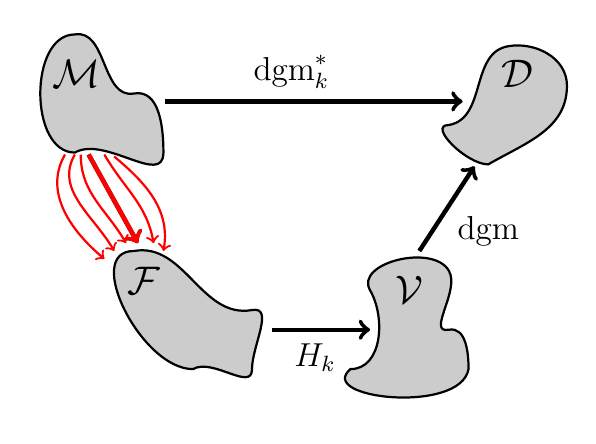
\begin{tikzpicture}[scale=0.5]

    \filldraw[thick, fill=black!20!white](-2,-1)
    to [out=10,in=190] (1,-2.5)
    to [out=10,in=90] (1,-4) 
    to [out=-90,in=30] (-0.5,-4)
    to [out=180, in=180] (-2,-1);
    
    
    \filldraw[thick, fill=black!20!white](6,-1.5)
    to [out=-60,in=190] (6,-3)
    to [out=10,in=90] (6.5,-4)
    to [out=-100,in=-140] (3.5,-4)
    to [out=0,in=-60] (4,-2)
    to [out=120, in=120] (6,-1.5); 
    
    
    \filldraw[thick, fill=black!20!white](-3.5,4.5)
    to [out=10,in=190] (-2,3)
    to [out=10,in=90] (-1.25,1.5) 
    to [out=-90,in=30] (-3.5,1.5)
    to [out=180, in=180] (-3.5,4.5); 
    
    
    \filldraw[thick, fill=black!20!white](6,2.2)
    to [out=10,in=190] (7.5,4.2)
    to [out=10,in=90] (9,3.2) 
    to [out=-90,in=30] (7,1.2)
    to [out=180, in=180] (6,2.2); 
    
    \draw[->, ultra thick] (-1.2,2.8) to (6.35,2.8);
    \draw[->, ultra thick] (-3.15,1.45) to (-1.9,-0.8);
    \draw[->, ultra thick](1.5,-3) to (4,-3);
    \draw[->, ultra thick] (5.25,-1) to (6.65,1.15);
    
    \node at (-3.45,3.5){\Large $\mathcal{M}$};
    \node at (-1.75,-1.75){\Large $\mathcal{F}$};
    \node at (5,-2){\Large $\mathcal{V}$};
    \node at (7.75,3.5){\Large $\mathcal{D}$};
    
    %\pause
    
    \node at (2,3.55){\large $\dgm_k^{\ast}$};
    \node at (2.6,-3.7){\large $H_k$};
    \node at (7,-0.5){\large $\dgm$};
        
    \draw[->, ultra thick, color=red] (-3.15,1.45) to (-1.9,-0.8);
    
    %\pause
    
    \draw[->, thick, color=red] (-3.75,1.45)
    to [out=240, in=140] (-2.75,-1.2);
    
    \draw[->, thick, color=red] (-3.5,1.45)
    to [out=240, in=120] (-2.5,-1);
    
    \draw[->, thick, color=red] (-3.35,1.45)
    to [out=270, in=120] (-2.2,-0.8);
    
    \draw[->, thick, color=red] (-2.75,1.45)
    to [out=-60, in=100] (-1.5,-0.8);
    
    \draw[->, thick, color=red] (-2.5,1.4)
    to [out=-40, in=80] (-1.25,-1);
    
    
\end{tikzpicture}
  
  
  \caption{This diagram shows the main pipeline of filtrations on pointclouds. The deep-red arrow represents the usual filtration used (\v{Cech} or Vietoris-Rips.) We want to find as many alternative red arrows as possible.}
\end{figure}


\section{Preliminaries}
For a finite set $X$, $\pow(X)$ denotes the set of all non-empty subsets of $X$. By $\mathcal{M}$ we will denote the collection of all finite metric spaces. Given a finite metric space $(X,d_X)$ we consider the map $\iota_X:\pow(X)\rightarrow \mathcal{M}$ given by $\sigma\mapsto (\sigma,d_X|_{\sigma\times \sigma})$, that is $\iota_X$ takes a  subset of $X$ and endows it with the restriction of the metric of $X$.
\facundo{Need to make the map $\iota_X$ explicit in many places in the paper.}
By the diameter $\diam(X)$ of a finite metric space $(X,d_X)$ we mean the number $\max_{x,x'\in X}d_X(x,x')$, and by the eccentricity function associated to $(X,d_X)$ we mean the function $\ecc_X:X\rightarrow \R_+$ such that $x\mapsto \max_{x'\in X}d_X(x,x').$


\defn{Given a metric space $(X,d_X)$ and a natural number $n$ consider the map $$\Psi_X^{(n)}:X\times \cdots\times X\rightarrow \R^{n\times n}$$ given by 
$$(x_1,\ldots,x_n)\mapsto \big(d_X(x_i,x_j)\big)_{i,j=1}^n.$$

Then, the \emph{$n$-th curvature set} of $(X,d_X)$ is the set 

$$\cset_n(X):=\im(\Psi_X^{(n)}).$$}

\defn{We define the diameter function to be $\diam:\M\rightarrow \R$ given by, 
$$ \diam(X)= \max_{x,x'\in X} d_X(x,x').$$
}
\defn{Let $X\in \M$. We define the eccentricity of a point $x^*\in X$ to be 
	$$ \ecc_X(x^*)= \max_{x\in X} d_X(x^*,x).$$}

\begin{thm}[\cite{dgh-props}]\label{thm:cset}
For any pair of compact metric spaces, and all $n\in\N$,  $$d_{\mathrm{H}}^{(\R^{n\times n}, l_\infty)}(\cset_n(X),\cset_n(Y))\leq 2 \, \dgh(X,Y).$$
\end{thm}

\defn{ Let $X$ be a finite set. A filtration on $X$ is any map $\psi_{X}:\pow(X) \rightarrow \R_+$ that satisfies the monotonicity condition: 
$$\psi_X(\tau)\leq \psi_X(\sigma) \hspace{1cm} \forall \, \, \tau\subset \sigma\subset X. $$}

It is possible to define a distance on filtered spaces $(X,F_X)$ as follows \cite{tripods}:

$$d_{\mathcal{F}}((X,F_X),(Y,F_Y)):= \inf_{Z,\phi_X,\phi_Y} \max_{\sigma \subset Z} |F_X(\phi_X(\sigma)) - F_Y(\phi_Y(\sigma ))|, $$

where $\phi_X$ and $\phi_Y$ are surjective maps from $Z$ to $X$ and $Y$ respectively. There is a result that can help us with the notion of stability:

\begin{thm}[\cite{tripods}]\label{thm:tripods}
For all finite filtered spaces $(X,F_X)$ and $(Y,F_Y)$, and all $k\in\mathbb{N}$ one has $$ \dB( \dgm_k^{}(X,F_X) , \dgm_k^{}(Y,F_Y) )\leq d_{\mathcal{F}}((X,F_X), (Y,F_Y)).$$
\end{thm}

%\zoe{To resolve the loaded local terminology, we can change the terminology to "base-point filtrations" and "$n$-local filtrations"}

\section{Global and Local Valuations}

When we apply the Vietoris Rips and and the \v{C}ech filtrations to view persistent homology barcodes, we are mapping from the category of finite metric spaces, $\M$, to the category of diagrams, $\mathcal{D}$. We must remember that map is a composition of three maps: the filtration functor, the homology functor, and then the bar code functor. From Theorem \ref{thm:cset}, we have nice stability between the category of filtration spaces to the category of diagrams. Thus, in our work we want to focus on filtration functors, and we want to both create new and rich families of filtration functors, and find stability results between the category of filtration spaces and the category of finite metric spaces. Towards this end, let us consider the following definitions:

\defn{Let $(X,d_X),(Y,d_Y)\in \M$ and $\psi: X\rightarrow Y$ such that $\forall x,x'\in X$, \\$d_X(x,x')\ge d_Y(\psi(x),\psi(x'))$. A \emph{filtration functor} is a map $\phi: \M\rightarrow \F$ such that for any $\sigma\in X$, we have that $\phi_X(\sigma)\ge\phi_Y(\psi(\sigma))$.\footnote{Plus other conditions.} \jose{Ultrametricity does not satisfy this last condition. It only satisfies monotonicity. Should we include this property despite this?}}

\defn{We say that a filtration functor $\phi:\M\rightarrow \mathcal{F}$ is $L$-stable if there exists $L>0$ such that:
$$L\: \dgh(X,Y)\geq d_{\mathcal{F}}((X,\phi_X),(Y,\phi_Y))$$ for all 
$X,Y\in\M.$}\\

One way in which we can define filtration functors is via the notion of valuations:

\facundo{(valuation may not be good name: better pre-valuation (?))}\jose{I agree.}
\defn{\label{def:valuations} A \emph{valuation} is a map $\nu_n:\pow(\R^{n\times n})\rightarrow \R_+$ such that $\nu_n$ is \emph{monotonic}, meaning that $\nu_n(A)\geq \nu_n(B)$ for all $B\subset A \in \pow(\R^{n\times n})$.}\\

We are interested in defining filtrations through valuations. The monotonicity condition is imposed so that the simplicial construction a valuation induces actually forms a simplicial complex. It assures that if a simplex is in the filtered space at a given time, all sub-simplices are also in the filtered space at that given time. 

\defn{A filtration functor $\phi:\M\rightarrow \F$ is \emph{$n$-local} for some $n\in \N$ if there exists some valuation $\nu_n:\pow(\R^{n\times n})\rightarrow \R_{+}$ such that $\forall \,X\in \M$ and $\forall \sigma\in X$, \\$$\phi_X(\sigma)=(\nu_n \circ \cset_n\circ \iota_X)(\sigma)$$} 

\facundo{I made the map $\iota_X$ appear explicitly above.}

\clm{\begin{enumerate}
\item Notice that if the filtration functor $\phi$ is $n$-local then it is $n'$-local for all $n'\geq n$. Thus by convention, when we say a filtration functor is $n$-local, we are referring to the minimal $n$.
\item The Vietoris-Rips functor is 2-local.  It follows from noticing that:
\begin{eqnarray*}
R_X(\sigma)&=& \diam(\sigma) \\
	&=& \max_{\{x,y\}\subset \sigma} d_X(x,y) \\
    &=& \max_{A\in K_2(\iota_X(\sigma) )}\max_{i,j}A_{ij}.
\end{eqnarray*}
What is happening is that the arrival time of a simplex under Vietoris-Rips depends only on pairwise distances between points in the simplex, which is information given by $\cset_2(\sigma)$. We can see that the valuation that generates the Rips filtration functor is $\nu_2(\mathcal{A})= \max\limits_{A\in \mathcal{A}} ||A||_{\infty}$ for all $\mathcal{A} \in \pow(\R^{2\times 2})$.

\item The \v{C}ech functor is not local. To show this, we construct a counterexample: \\Let $(P,d_P)$ be the space of three equidistant points $P=\{p_1,p_2,p_3 \}$ with distance 2 and $(Q,d_Q)$ be the tree-space of four points $Q=\{q_0,q_1,q_2,q_3\}$ given by the matrix:
$$d_Q= \begin{pmatrix}
	0 & 1 & 1 & 1 \\
    1 & 0 & 2 & 2 \\
    1 & 2 & 0 & 2 \\
    1 & 2 & 2 & 0 \\
\end{pmatrix}$$
Since the subset $A=\{q_1,q_2,q_3\}\subset Q$ and $P$ are isometric, $\cset_n(A)= \cset_n(P)$ for all $n\in \N$. If the \v{C}ech functor was $n$-local for some $n\in \N$, then, 
$$C_Q(A)= \nu_n(\cset_n(A))= \nu_n(\cset_n(P))= C_P(P).$$
For some $n\in \mathbb{N}$. But $C_X(A)= 1$ since $\cap_{i=1}^n B(q_i,1)=\{q_0\}$ and $C_Y(P)=2$, which holds a contradiction. The intuitive explanation why the \v{C}ech complex construction is not $n$-local for some $n\in \N$ is that the arrival time of a simplex depends on properties of the whole space, and not only on the metric properties of the points in the simplex.

\end{enumerate}}

\defn{Let $n\in\mathbb{N}$ and let  $\nu_n: \mathrm{pow}(\mathbb{R}^{n\times n })\rightarrow \mathbb{R}$ be a valuation. Given $L\geq 0$, we will say that $\nu_n$ is $L-$stable if and only if for all non-empty  $A,B\subset \R^{n\times n}$:
 $$ |\nu_n(A)-\nu_n(B)|\leq L \,\dH^{(\mathbb{R}^{n\times n}, l_\infty)}( A, B )$$}


Stability is a desirable property, since it relates the notion of distance in $\M$ to distance in the space of barcodes. Given Theorem \ref{thm:tripods}, and recalling the stability of the $\cset_n$ map (cf. Theorem \ref{thm:cset}), then we get the following:

\begin{cor}\label{lstablevaluation} Let $\nu_n$ be any $L$-stable valuation. Then, for all $X,Y\in\M$ and $k\in\mathbb{N}$ one has
 $$2\,L\,\dgh(X,Y) \geq \dB\left( \dgm_{k}^{\nu_n \circ \cset_n}(X),\dgm_{k}^{\nu_n \circ \cset_n}(Y) \right). $$
\end{cor}
\begin{proof}
Let $X,Y\in \M$. Let $R\subset X\times Y$ be the correspondence that attains the Gromov-Hausdorff distance between this two spaces, $\dgh(X,Y)=\frac{1}{2}\dis(R)$. Now, we define the maps $\pi_1:R\rightarrow X$ and $\pi_2: R\rightarrow Y$ the natural projections from $R$ to $X$ and $Y$ respectively. From the fact that $R$ is a correspondence it follows that $\pi_1$ and $\pi_2$  are surjective. 

For this, first notice that the tripod $(R,\pi_1,\pi_2)$ consists of a set $R$, and two surjections from $R$ to $X$ and $Y$ respectively. Now, let $S\subset R$. It is worth noticing that $S$ is a correspondence between $\pi_1(S)$ and $\pi_2(S)$. Considering $\pi_1(S)\subset X$ and $\pi_2(S)\subset Y$ with the induced subspace metric from $X$ and $Y$ respectively, it follows that,
'
\begin{eqnarray*}
|\nu_n\circ \cset_n(\pi_1(S))-\nu_n\circ \cset_n(\pi_2(S))|&\leq & L \,\dH(\cset_n(\pi_1(S)), \cset_n(\pi_2(S)))\\
  &\leq& 2L\,\dgh(\pi_1(S),\pi_2(S)).\\  
\end{eqnarray*}

Since $S$ is a correspondence between $\pi_1(S)$ and $\pi_2(S)$ and $S\subset R$ then
\begin{eqnarray*}
\dgh(\pi_1(S),\pi_2(S))&\leq &\frac{1}{2} \dis(S)\\
	&=& \frac{1}{2}\max_{(x,y),(x',y')\in S} |d_X(x,x')-d_Y(y,y')|\\
	&\leq& \frac{1}{2}\max_{(x,y),(x',y')\in R} |d_X(x,x')-d_Y(y,y')|\\
    &=& \dgh(X,Y).
\end{eqnarray*}

It follows that for all $S\subset R$, 

$$ |\nu_n\circ \cset_n(\pi_1(S))-\nu_n\circ \cset_n(\pi_2(S))|\leq 2L\, \dgh(X,Y).$$

We conclude that $d_{\F}((X,(\nu_n\circ \cset_n)_X),(Y,(\nu_n\circ \cset_n)_Y))\leq 2L\,\dgh(X,Y).$ From  \ref{thm:tripods},  
\begin{eqnarray*}
\dB(\dgm^{\nu_n\circ\cset_n}_k(X), \dgm^{\nu_n\circ\cset_n}_k(Y))&\leq & d_{\F }((X,(\nu_n\circ \cset_n)_X),(Y,(\nu_n\circ \cset_n)_Y))\\
&\leq & 2L\dgh(X,Y).
\end{eqnarray*}
\end{proof}


\section{Basepoint Filtration Functors}

%\facundo{In this section: Need to fix notation in many places.}

\defn{For any $X\in \M$, a family of \emph{basepoint filtrations} are: \\$\{\psi_X(x_0):\pow (X) \rightarrow \R \}_{x_0\in X}$ where for all $x_0\in X$, $\psi_X(x_0)$ is a filtration on $X$. We call $X$ the base space of this basepoint filtrations}.\\

With a basepoint filtration, instead of choosing a single filtration for the space, we have a different way of filtrating for each point in it.

\defn{A \emph{basepoint filtration functor} is a map $\Psi:\M \rightarrow \pow(\F)$, such that $\Psi$ takes any $X\in \M$ to a family of basepoint filtrations $\Psi(X)= \{\psi_X(x_0): \pow(X) \rightarrow \R \}_{x_0\in X}$.}\\

A basepoint filtration functor gives a method of basepoint filtrating each space. Note that any filtration we have previously defined in the general sense can be considered as a basepoint filtration as well: 


\begin{ex}
Let $\psi:\M \rightarrow \F$ be any filtration functor. We define the basepoint filtration functor $\Psi^{b}: \M \rightarrow \pow(\F)$ to be,
	$$\psi^b_X(x_0)= \psi_X \hspace{1cm} \forall \, X\in \M, \, x_0\in X.$$
\end{ex}

\begin{ex}\label{eccfiltration}
Another more interesting example of a basepoint filtration functor is $$\Psi^\ecc: \M \rightarrow \pow(\F)$$
Such that for all $X\in \M$,
$$\Psi^\ecc(X) = \{\psi_X(x_0):\pow(X)\rightarrow \R\}_{x_0\in X},$$ 
where for $x\in X$ and $\sigma \subset X$, $$\psi_X(x_0)(\sigma) := \max \left\{\diam(\sigma),\frac{1}{2}\left(\ecc_X(x_0)-\min_{x'\in \sigma}d_X(x_0,x')\right)\right\}.$$
\end{ex}

\begin{prop}
For each $x\in X$ and $y\in Y$ let, 
$$C_{\Psi^\ecc}(x,y) := \dB(\dgm_k(\psi_X(x)),\dgm_k(\psi_Y(y))).$$

Then, 

$$2\dgh(X,Y) \geq \min_R \max_{(x,y)\in R}C_{\Psi^\ecc}(x,y).$$
\end{prop}
\begin{proof}
%\facundo{exercise}
Let $\dgh(X,Y) = \eta$, and let $R_0 \subset X \times Y$ be a correspondence such that $\dis(R_0) = 2 \eta$. We will show that $\dis(R_0) \geq d_\mathcal{F}((X,\psi_X),(Y,\psi_Y))$. To do this, we will use the definition for $d_\mathcal{F}((X,\psi_X),(Y,\psi_Y))$ from the preliminaries. 

Let $Z=R_0$ and let $\phi_X$ and $\phi_Y$ be the projections from $R_0$ down to $X$ and $Y$, respectively. Pick base-points $x$ and $y$ such that $(x,y)\in R_0$. Then we have: 

$$d_\mathcal{F}((X,\psi_X(x)),(Y,\psi_Y(y))) \leq \max\limits_{\sigma \subset R_0}|\psi_X(x)(\phi_X(\sigma)) - \psi_Y(y)(\phi_Y(\sigma))|.$$

Denote $\phi_X(\sigma) = \sigma_X$ and $\phi_Y(\sigma) = \sigma_Y$  and we see:

\jose{How should we handle this equation... it is too long for parenthesis to be adjusted. I guess that breaking each line into two. Maybe it is a good idea to define a function through which we can resume the expression.}

$$\max\limits_{\sigma \subset R_0}|\psi_X(x)(\phi_X(\sigma)) - \psi_Y(y)(\phi_Y(\sigma))| =$$

$$\max_{\sigma \in R_0}|\psi_X(x)(\sigma_X)-\psi_Y(y)(\sigma_Y)| = $$

$$\max_{\sigma \in R_0}|\max\{\diam(\sigma_X),\frac{1}{2}(\ecc_X(x)-\min_{x'\in \sigma_X}d_X(x,x'))\} - \max\{\diam(\sigma_Y),\frac{1}{2}(\ecc_Y(y)-\min_{y'\in \sigma_Y}d_Y(y,y'))\}| \leq$$

$$\max_{\sigma \in R_0}|\max\{\diam(\sigma_X)-\diam(\sigma_Y), \frac{1}{2}(\ecc_Y(y)-\min_{y'\in \sigma_Y}d_Y(y,y')) - \frac{1}{2}(\ecc_X(x)-\min_{x'\in \sigma_X}d_X(x,x'))\}.$$

Now fix $\sigma \in R_0$ and I will show that for $\sigma$, this quantity is less than or equal to $2\eta$. To do this, the proof is split into two cases:\\

\textbf{Case 1:} This maximum is $\diam(\sigma_X)-\diam(\sigma_Y).$\\
Since $\sigma = [(x_1,y_1),...,(x_n,y_n)]$ for some $n \in \mathbb{N}$ we have for some $(x_i,x_j) \in \sigma_X$, $\diam(\sigma_X) = d_X(x_i,x_j)$. Then:

$$\diam(\sigma_X)-\diam(\sigma_Y) = d_X(x_i,x_j) - \diam(\sigma_Y) \leq d_X(x_i,x_j) - d_Y(y_i,y_j) \leq 2\eta.$$

Following a symmetric proof gives $\diam(\sigma_Y)-\diam(\sigma_X) \leq 2\eta$, so putting these together gives us the desired $|\diam(\sigma_X)-\diam(\sigma_Y)|\leq 2\eta$.\\

\textbf{Case 2:} This maximum is $\frac{1}{2}(\ecc_Y(y)-\min\limits_{y'\in \sigma_Y}d_Y(y,y')) - \frac{1}{2}(\ecc_X(x)-\min\limits_{x'\in \sigma_X}d_X(x,x')).$\\
Here we have,

$$\left|\frac{1}{2}\left(\ecc_X(x)-\min\limits_{x'\in \sigma_X}d_X(x,x')\right) - \frac{1}{2}\left(\ecc_Y(y)-\min\limits_{y'\in \sigma_Y}d_Y(y,y')\right)\right| =$$

$$\frac{1}{2}\left|(\ecc_X(x)-\ecc_Y(y)) + \left(\min\limits_{y'\in \sigma_Y}d_Y(y,y') - \min\limits_{x'\in \sigma_X}d_X(x,x')\right)\right| \leq$$

$$\frac{1}{2}\left(\left|\ecc_X(x)-\ecc_Y(y)\right| + \left|\min\limits_{y'\in \sigma_Y}d_Y(y,y') - \min\limits_{x'\in \sigma_X}d_X(x,x')\right|\right).$$\\

Now we have let $x'\in X$ such that $\ecc_X(x) = d_X(x,x')$. Then if $(x,y),(x',y')\in R_0$, We have:

$$\ecc_X(x)-\ecc_Y(y) = d_X(x,x') - \ecc_Y(y) \leq d_X(x,x')-d_Y(y,y') \leq 2\eta,$$

and via similar argument, $\ecc_Y(y)-\ecc_X(x) \leq 2\eta$. It follows that, 

$$|\ecc_X(x) - \ecc_Y(y)|\leq 2\eta.$$\\

For the second half, let $x'\in \sigma_X$ such that $x'$ is $\min\limits_{x'\in \sigma_X}d_X(x,x')$ and let $y'$ be such that $(x',y')\in R_0$. Then we have:

$$\min_{y'\in \sigma_Y}d_Y(y,y') - \min_{x'\in \sigma_X}d_X(x,x') = \min_{y'\in \sigma_Y}d_Y(y,y') - d_X(x,x') \leq d_Y(y,y') - d_X(x,x') \leq 2\eta$$

and via similar argument, 

$$\min_{x'\in \sigma_X}d_X(x,x')-\min_{y'\in \sigma_Y}d_Y(y,y') \leq 2\eta.$$

So putting these together, we get:



$$\left|\min_{y'\in \sigma_Y}d_Y(y,y') - \min_{x'\in \sigma_X}d_X(x,x')\right|\leq 2\eta.$$

Returning to the start, we now have:

$$\left|\frac{1}{2}\left(\ecc_X(x)-\min\limits_{x'\in \sigma_X}d_X(x,x')\right) - \frac{1}{2}\left(\ecc_Y(y)-\min\limits_{y'\in \sigma_Y}d_Y(y,y')\right)\right| \leq $$

$$\frac{1}{2}\left(\left|(\ecc_X(x)-\ecc_Y(y))\right| + \left|(\min\limits_{y'\in \sigma_Y}d_Y(y,y') - \min\limits_{x'\in \sigma_X}d_X(x,x'))\right|\right) \leq $$

$$\frac{1}{2}(2\eta + 2\eta) \leq 2\eta.$$

Now we have shown that for any $\sigma \in R_0$ that:

$$\bigg|\max\bigg\{\diam(\sigma_X),\frac{1}{2}\left(\ecc_X(x)-\min_{x'\in \sigma_X}d_X(x,x')\right)\bigg\} \hspace{3cm}$$
$$\hspace{3cm} - \max\bigg\{\diam(\sigma_Y),\frac{1}{2}\left(\ecc_Y(y)-\min_{y'\in \sigma_Y}d_Y(y,y')\right)\bigg\}\bigg| \leq 2\eta \implies$$

$$\max_{\sigma \in R}\bigg|\max\bigg\{\diam(\sigma_X),\frac{1}{2}\left(\ecc_X(x)-\min_{x'\in \sigma_X}d_X(x,x')\right)\bigg\} \hspace{3cm}$$
$$\hspace{3cm} - \max\bigg\{\diam(\sigma_Y),\frac{1}{2}\left(\ecc_Y(y)-\min_{y'\in \sigma_Y}d_Y(y,y')\right)\bigg\}\bigg| \leq 2\eta.$$

Now we have :

$$d_\mathcal{F}((X,\psi_X(x)),(Y,\psi_Y(y))) \leq 2\eta.$$

Finally, by Theorem \ref{thm:tripods}, for any $(x,y) \in R_0$ we have:

$$\dB( \dgm_k(X,\psi_X(x)) , \dgm_k(Y,\psi_Y(y))\leq 2\dgh(X,Y).$$

Since this was dealing with $R_0$ we conclude that,

\begin{eqnarray*}
\min_R\max_{(x,y)\in R}\dB\left( \dgm_k(X,\psi_X(x)) , \dgm_k(Y,\psi_Y(y)\right) &\leq & \max_{(x,y)\in R_0}\dB\left( \dgm_k(X,\psi_X(x)) , \dgm_k(Y,\psi_Y(y))\right)\\
&\leq & 2\dgh(X,Y).
\end{eqnarray*}



\end{proof}


% \facundo{(I wonder if the material below can be salvaged by making more assumptions on the underlying spaces..)}

% \defn{Given $\psi_X:X\rightarrow \F(X)$ and $\psi_Y:Y\rightarrow \F(Y)$, an $\epsilon$ matching between metric spaces $X$ and $Y$ is a partial bijection 
% $\sigma:X\rightarrow Y$, where $domain(\sigma) = X' \subset X$,  $codomain(\sigma) = Y' \subset Y$ and $|X'| = |Y'|$, if:\\
% \begin{enumerate}
% \item $\forall x\in X\setminus X', \ pers(\dgm(\psi_X(x)))\leq 2\epsilon$

% \item $\forall y\in Y\setminus Y', \ pers(\dgm(\psi_Y(y)))\leq 2\epsilon$ 

% \item $\forall k \in \mathbb{N}$ and $\forall x\in X', \  \dB(\dgm_k(\psi_{X'}(x)),\dgm_k(\psi_{Y'}(\sigma(x)))) \leq \epsilon$
% \end{enumerate}}

% We wish to show that this formulation of an $\epsilon$-matching "fits" nicely, that is we wish to show:
% $$2\dgh(X,Y)\stackrel{(1)}{\geq} \min\{\epsilon \geq 0 : \exists \sigma : X \rightarrow Y, \sigma \ is \ an \ \epsilon - matching\} \stackrel{(2)}{\geq} \min_R \max_{(x,y)\in R}C(x,y)  $$

% Proof of (2): Let $(X,d_X),(Y,d_Y)$ be two finite metric spaces, and let $\min\{\epsilon \geq 0 : \exists \sigma : X \rightarrow Y, \sigma \ is \ an \ \epsilon - matching\} = \epsilon '$ Then let $\sigma:X'\rightarrow Y'$ be an $\epsilon '$-matching.\\
% Now take $R\subset X\times Y$, a correspondence such that the elements $(x,y) \in R$ are either of the form $(x,\sigma(x))$ if $x\in X'$ or $(x,y)$ if $x \not\in X'$ and $y \not\in Y'$. Now let $(x,y)\in R$ and we will consider $C(x,y)$. We have:
% $$C(x,y) = \dB(\dgm_k(\psi_X(x)),\dgm_k(\psi_Y(y)))$$
% I will show that this value $C(x,y) \leq \epsilon '$, which will complete the proof of (2). We have that $C(x,y) = \min\limits_\mathcal{P}\M(\mathcal{P})$. Let $\mathcal{P}$ be the partial matching induced by $\sigma$. Then we have:
% $$\M(\mathcal{P}) = \max \{\max_{x\in X'}||(b_x,d_x)-(b_{\sigma(x)},d_{\sigma(x)})||_\infty,\max_{x \in X \setminus X'}\frac{1}{2}pers(b_x,d_x), \max_{y \in Y \setminus Y'}\frac{1}{2}pers(b_y,d_y)\}$$
% By the conditions for the $\epsilon '$-matching we know that $\max\limits_{x \in X \setminus X'}\frac{1}{2}pers(b_x,d_x) \leq \epsilon '$ and likewise, 
% $\max\limits_{y \in Y \setminus Y'}\frac{1}{2}pers(b_y,d_y) \leq \epsilon '$
% Now the remaining term left to bound is \\$\max\limits_{x\in X', y\in Y'}||(b_x,d_x)-(b_y,d_y)||_\infty$. Notice that in general,: 
% $$\max\limits_{x\in X'}||(b_x,d_x)-(b_{\sigma(x)},d_{\sigma(x)})||_\infty \geq \dB(\dgm_k(\psi_{X'}(x)),\dgm_k(\psi_{Y'}(\sigma(x))))$$
% However, $\dB(\dgm_k(\psi_{X'}(x)),\dgm_k(\psi_{Y'}(\sigma(x))))$ is induced by some partial matching $\mathcal{P}''$ between subsets of $X'$ and $Y'$. If we call $\mathcal{P}'$ the restriction of our $\mathcal{P}$ to $X'$ and $Y'$, then if we alter our $\mathcal{P}$ by changing its restriction to $X'$ and $Y'$ from $\mathcal{P}'$ to $\mathcal{P}''$, then we get that:
% $$\M(\mathcal{P}) \leq \max\{\dB(\dgm_k(\psi_{X'}(x)),\dgm_k(\psi_{Y'}(\mathcal{P}(x)))), \max_{x \in X \setminus X'}\frac{1}{2}pers(b_x,d_x), \max_{y \in Y \setminus Y'}\frac{1}{2}pers(b_y,d_y)\} \leq \epsilon '$$

% \facundo{One idea that just came to mind in oder to test whether (1) and (2) above may hold: consider $X$ and $Y$ to be tree metric spaces and $k=0$.}

\subsection{A general description}
Define the basepoint $n$-curvature set of the metric space $X$ as follows: for each $x_0\in X$, let 
$$ \cset_n(x_0,X) :=  \mathrm{im}\big(\Psi^{(n+1)}_X(x_0,\cdot)\big) \subset \R^{(n+1)\times (n+1)}.$$
Consider the projection $\pi_n:\R^{(n+1)\times (n+1)}\rightarrow \R^{n\times n}$ given by 
$$\big(a_{ij}\big)_{i,j=1}^{n+1}\mapsto \big(a_{ij}\big)_{i,j=2}^{n+1}$$
Notice that for every $x_0\in X$ one has $\pi_n(\cset_n(x_0,X)) = \cset_n(X).$

Given a natural number $n$ and any stable valuation $\nu_{n+1}$ one can construct the following family of basepoint filtrations:
$$x\mapsto \nu_{n+1}\circ K_n(x_0,\cdot).$$


\facundo{all vertical bars $|$ below should be bigger: they should span the WHOLE vertical space of the symbols between them. Use for example} \begin{verbatim}\big\end{verbatim}

\begin{ex}
\nate{still working on what the best way to deal with the extra constant is}
\jose{I think that the ecc-filt can't be basepoint local, since it depends on $\ecc(x_0)$, which is a global property of $x_0$ with respect to the space.}
We show how the functor from (\ref{eccfiltration}) also satisfies this formulation of a basepoint functor. To refresh, we have 

$$\psi_X(x)(\sigma) = \max\left\{\diam(\sigma),\frac{1}{2}\left(\ecc_X(x)-\min_{x'\in \sigma}d_X(x,x')\right)\right\}$$

Now we have $\cset_n(x,X)$ and need to find $\nu_{n+1}:pow(\mathbb{R}^{(n+1) \times (n+1)})\rightarrow \mathbb{R}$. If we let:\\
$$\nu_{n+1} = \max_{A\in K_n(x,X)}\left\{\max_{2\leq i,j\leq n+1}(a_{ij}),\frac{1}{2}\left(\ecc_X(x)-\min_{j=1}(a_{ij})\right)\right\}$$
Then we see that this is the desired $\nu_{n+1}$ which satisfies 

\end{ex}

\begin{thm}
\label{thm:kn-local}
Let $\nu_{n+1}:pow(\R^{(n+1)\times(n+1)})\rightarrow \R$ be an L-stable valuation. Then for all $n \in \mathbb{N}$, $\forall\, k \in \mathbb{N}$ we have: $$2L\,\dgh(X,Y) \geq \min_{R}\max_{(x,y)\in R}\dB\left( \dgm_{k}^{\nu_{n+1} \circ \cset_n(x,\cdot)}(X),\dgm_{k}^{\nu_{n+1} \circ \cset_n(y,\cdot)}(Y) \right).$$

\end{thm}

\begin{proof}[Proof of Theorem \ref{thm:kn-local}]
Let $(X,d_X),(Y,d_Y)\in \M$. Then fix $R \subset X\times Y$ such that\\ $\dis(R) = \eta = 2\dgh(X,Y)$. Now fix some $(x,y) \in R$, and I will first show an analog of \ref{thm:cset}, which is:
$$\dH^{(\R^{n\times n},l_\infty)}(\cset_n(x,X),\cset_n(y,Y))\stackrel{(1)}\leq 2 \, \dgh(X,Y)$$
We have that $$\dH^{(\R^{n\times n},l_\infty)}(\cset_n(x,X),\cset_n(y,Y)) = $$
$$\max\left\{\max\limits_{A\in \cset_n(x,X)}\min\limits_{B\in \cset_n(y,Y)}||A-B||_\infty, \max\limits_{B\in \cset_n(y,Y)}\min\limits_{A\in \cset_n(x,X)}||B-A||_\infty\right\}.$$

Now let $A\in \cset_n(x,X)$ be given. This is a matrix generated by the distances between $n+1$ points in $X$, denote them $x,x_1,...x_n$. We can then take $B\in \cset_n(y,Y)$ to be the distance matrix generated by the points $y,y_1,...,y_n$  in $Y$ where for all $1\leq i \leq n$, $(x_i,y_i)\in R$. Then we have $||A-B||_\infty \leq \eta$. Thus, 
$\max\limits_{A\in \cset_n(x,X)}\min\limits_{B\in \cset_n(y,Y)}||A-B||_\infty \leq \eta.$
Through a similar process given any $B\in \cset_n(y,Y)$ one can pick points in $X$ so that they generate a distance matrix $A$ where 
$\max\limits_{B\in \cset_n(y,Y)}\min\limits_{A\in \cset_n(x,X)}||B-A||_\infty \leq \eta.$ 
So, we are left with 

$$\max\left\{\max\limits_{A\in K_n(x,X)}\min\limits_{B\in K_n(y,Y)}||A-B||_\infty, \max\limits_{B\in K_n(y,Y)}\min\limits_{A\in K_n(x,X)}||B-A||_\infty\right\} \leq \eta.$$
And the desired inequality (1) is shown.
From here the remainder of the proof follows the same as the proof of Corollary \ref{lstablevaluation}.

\end{proof}


\section{A theorem about existence of rich families}


% \defn{A functor $\phi$ is stable if whenever we have $(X,d_X),(Y,d_Y)\in \M$ and a tripod $\{Z \twoheadrightarrow X, Z \twoheadrightarrow Y\}$, with maps $\phi_X:Z \twoheadrightarrow X$ and $\phi_Y:Z \twoheadrightarrow Y$, then $$dis_\M(R,d_X,d_Y) \geq dis_\F(R, \phi_X,\phi_Y).$$}

We still have our motivation of finding a filtration where the bottleneck distances between the barcodes of two spaces attains the Gromov-Hausdorff distance for any pair of finite metric spaces. This has been unsuccessful when considering any single filtration, so instead we ask: is it possible to find a family $(\Phi_\alpha)_{\alpha}$ of filtration functors such that for every pair of spaces $X,Y\in \M$ there is a functor $\Phi_\alpha$ such that this particular functor attains the Gromov-Hausdorff distance through the bottleneck distance? This idea is developed in the following theorem.

\begin{thm}
There exists $\Phi$, a family of stable filtration functors such that for all $(X,d_X),(Y,d_Y) \in \M$, we have 
$$\dgh(X,Y) = \frac{1}{2}\sup\limits_{\phi \in \Phi}\dB\left(\dgm_0(\phi_X),\dgm_0(\phi_Y)\right).$$
\end{thm}
\jose{Check the def. of bottleneck to verify the constant that we are adding to the theorem.}
\begin{proof}
For each $Z\in\M$ we can define the canonical filtration functor $Q(Z):\M\rightarrow \F$ given by $X\mapsto Q(Z)_X$ where,
$$ Q(Z)_X(\sigma) = \dgh(X,Z), \hspace{1cm} \forall \sigma\subset X \in \M. $$

This filtration yields an empty space on the interval $[0,\dgh(X,Z))$ and has the complete simplicial complex in $[\dgh(X,Z),\infty)$. Then, $$\dgm_0(Q(Z)_X)=\left\{[\dgh(X,Z),\infty)\right\}.$$
Thus, $$\dB(\dgm_0(Q(Z)_X),\dgm_0(Q(Z)_Y))=|\dgh(X,Z)-\dgh(Y,Z)|.$$ 

From the triangle inequality on $\M$ it follows that,
$$\dB(\dgm_0(Q(Z)_X),\dgm_0(Q(Z)_Y))=|\dgh(X,Z)-\dgh(Y,Z)|\leq \dgh(X,Y),$$
for all $X,Y,Z \in \M$. Since $\dgh(Y,Y)=0$,
$$ \dB(\dgm_0(Q(Y)_X),\dgm_0(Q(Y)_Y))= \dgh(X,Y) \hspace{1cm} \forall X,Y \in \M.$$
We conclude that,
$$\dgh(X,Y)= \sup_{Z\in\M}\dB(\dgm_0(Q(Z)_X),\dgm_0(Q(Z)_Y)) \hspace{1cm} \forall X,Y \in \M.$$
\end{proof}

So now we have a family that satisfies the desired property. The problem we face is that the construction shown needs previous knowledge of the Gromov-Hausdorff distance. This indicates that the family we built in the proof is not useful in terms of computation. The positive side is that it guarantees the existence of families of this nature.

\section{Characterization results for valuations}
If we consider the possible functions $\nu$ within our definition of $n$-local, what are the constraints on $\nu$ that we can look at to construct potential filtration functors?

Consider first $\nu: \pow(\R)\rightarrow \R$. We see the following constraints:
\begin{enumerate}
\item $\forall a\in \R, \nu(\set{a}) = a$

\item $\nu$ monotonic

\item $\nu(A\cup B)\le \max(\nu(A),\nu(B)) \hspace{1cm} \forall A,B\in \pow(\R)$
\end{enumerate}
Now if we want to generalize this map $\nu:\pow(\R)\rightarrow \R$ to a map $\nu:\pow(\R^{n\times n})\rightarrow \R$, there are two natural cases to look at:

$\eta:\pow (\R^n)\rightarrow \R^n$
\begin{enumerate}
\item How do we compare $\eta(A)$ and $\eta(B)$? element wise ordering? (element wise doesn't seem to work, can we come up with a rigorous notion of comparing them


\item $\eta(\set{\vec{w}})=w\in\R^n$

\item $\eta(A\cup B)\le \max(\eta(A),\eta(B)$

\end{enumerate}

$\eta:\pow(\R^n)\rightarrow \R$
\begin{enumerate}
\item monotonic and we have a rigorous notion of $\eta(A)\le \eta(B)$ from mapping into $\R$

\item $\eta(\set{\vec{w}})=||\vec{w}||$ for $\vec{w}\in\R^n$ $\ast\ast$

\item $\eta(A\cup B)\le \max(\eta(A),\eta(B))$
\end{enumerate}

While considering $\ast\ast$, however, we notice that there are many different constraints that could relax the constraints placed on our filtration functors. Such as considering $M(A)=\left[ \vec{w_1}| \dots|\vec{w_n}\right]$ the matrix that is all the vectors in $A$ concatenated in a matrix. This then allows us to take determinants and Frobenius norms and others. We can also maximize by entry.


After verifying this result, the following was discussed:
/
\begin{center}
{\it	Let $\nu: \pow(\mathbb{R}^{n}) \rightarrow \mathbb{R}$ a valuation. Is it always possible to find $\gamma: \pow(\mathbb{R}^{n})\rightarrow \pow(\mathbb{R})$ and $\mu:pow(\mathbb{R})\rightarrow \mathbb{R} $ such that $\nu= \mu\circ \gamma $?}
\end{center}

We studied various examples of possible alternatives. First, we tried to define:

  $$ \nu_n(A)= \min_{p\in \mathbb{R}^n} \max_{a\in A}|| p-a||_{\infty}.$$

It was possible to prove that this particular valuation can be expressed as the composition of two maps. Mainly it was possible because we were using the $l^{\infty}-$norm, and the optimal ends up being an entrywise optimal. 

We also discussed the following distances, trying to understand if they were suitable to factorization or not:

\begin{eqnarray*}
	\nu_1(A)&=& \dH(\{p,q\}, A ), \hspace{1cm} p,q\in \mathbb{R}^n. \\
    \nu_2(A)&=& \min_{p,q\in \mathbb{R}^n} \dH(\{p,q\},A).
\end{eqnarray*}

A worth mentioning observation is that, in general is possible to factorize a valuation through the following:
$$ \nu(A)= \max (-\infty, \nu(A)], \hspace{1cm} \forall A \subset \mathbb{R}^n. $$
    This indicates that it is reasonable to impose some restrictions to the maps $\gamma$ and $\mu$ to avoid this trivial factorization.  

 
 We can define a $k$-point functor that takes the Hausdorff distance between a set of $k$ points and the metric space. This filtration does not factor naturally through $\pow{\R}$ but instead $\pow{\R^k}$, as long as we impose the following conditions on $\mu$ and $\gamma$ which are desirable conditions for $\mu$ and $\gamma$ to have.

\defn{Let $\gamma:X^n\rightarrow \pow{\R^k}$ be a map such that $\gamma$ takes each coordinate in $X^n$ to a single element with =in a set in $\pow{\R^k}$}

\defn{Let $\mu:\pow{\R^k}\rightarrow \R$ be a map such that $\mu$ only takes a composition of maximums and minimums }

We can more precisely define our $\mu$ and $\gamma$ for such a functor as follows:

$$\gamma: X^n\rightarrow \pow(\R^k)$$
$$\gamma_a: a\mapsto (||a-p_1||,\dots, ||a-p_k||)$$
$$\gamma(A)=\cup_{a\in A} \gamma_a(a)$$

$$\mu:\pow(\R^k)\rightarrow \R$$
$$\mu: B \mapsto \max(\max(\min_{b\in B}(b)),\max_{i\in[k]}(\min_{b\in B}(b_i)))$$

%The $\mu$ and $\gamma$ then work as a factorization as we can see below:


\ex{The following two equivalent definitions give us the 2-point functor

$$f_A(p,q)=d_{\mathrm{H}}(\set{p,q},A),$$    $$f_A(p,q)=\max\left(\max_{a\in A}(\min(||p-a||,||q-a||)),\max\left(\min_{a\in A}(||p-a||),\min_{a\in A}(||q-a||)\right)\right)$$. 

In general, the furthest $\gamma$ can go with information is to somehow use just the distances that are $||p-a||$ and $||q-a||$. Next we can see that when we get to this information we somehow need to keep track of whether a distance is from $p$ or $q$. Thus it is a natural notion that for each $a$ we can map $a$ to a pair of ordered points in $\R^2$ where the first is the distance from $p$ and the second, the distance from $q$. We can notice that if we go from $A$ into the set $\pow(\R^2)$ then we can easily define a $\mu$ that is just a composition of maximum and minimum functions. 

Let's take $\gamma$ and $\mu$ to be defined as follows:

$$\gamma: X^n\rightarrow \pow(\R^2)$$
$$\gamma_a: a\mapsto (||a-p||,||a-q||)$$
$$\gamma(A)=\cup_{a\in A} \gamma_a(a)$$

$$\mu:\pow{\R^2}\rightarrow \R$$
$$\mu: B \mapsto \max(\max(\min_{b\in B}(b)),\max(\min_{b\in B}(b_1),\min_{b\in B}(b_2)))$$


%------------------------

\section{Characterization Results for Valuation (v2)}
Recall definition \ref{def:valuations}. 


$f_p(A)=\max_{a\in A}||a-p||_{\infty}$

$\hat{F}_1(A)=\min_{p\in \R^n}f_p(A)$



%-----------------------------------------------------------------------------------------

\section{Specific Examples of Functors with Data}


\subsection{Filtrations based on ultrametricity}
\facundo{whenever using $\sigma\subset X$, for $X$ a f.m.s., as metric space we need to use map $\iota_X$.}

We can define a filtration based on ultrametricity, meaning based on how close a simplex or space is from being ultrametric.

We will define the ultrametric deviation function to be:
$$ \ud(x_1,x_2,x_3)= d_{X}(x_1,x_2)- \max\{d_X(x_1,x_3),d_X(x_2,x_3)\}, \hspace{1cm} \forall x_1,x_2,x_3\in X. $$

This function is measuring how much a triangle $(x_1,x_2,x_3)$ fails to be an ultrametric triangle. Then, we can define the ultrametricity of a metric space to be:

$$ \ult(X)= \max_{x_1,x_2,x_3\in X} \ud(x_1,x_2,x_3), \hspace{1cm} \forall X\in \mathcal{M}.$$

Once this is defined, we can define the filtration functor $\ult^*$ to be,

$$\ult^*_X(\sigma) = \ult(\iota_X(\sigma) ),\hspace{1cm} \forall \, \sigma \subset X,$$

considering the subspace metric of $\sigma$ induced by $X$. Now, there are some observations worth making:
\begin{itemize}
\item Indeed this is a filtration: if $\tau\subset \sigma$ then $\ult(\tau)\leq \ult(\sigma)$. Then, for all $r\geq 0$, the space $U_r(X)$ is a simplicial complex.

\item The filtration functor $F$ is $3$-local, induced by the valuation:
$$ \nu_3: \pow(R^{n\times n}) \rightarrow \F,$$
$$ A \longmapsto  \max_{a\in A} (a_{12}-\max\{a_{13}, a_{23} \}).$$

\item The valuation $\nu_3$ is $2-$stable. It follows from the general stability theorem that for all $k\in \N\cup \{0\}$:
$$4\, \dgh(X,Y)\geq \dB\left(\dgm^{\ult^*}_{k}(X), \dgm^{\ult^*}_{k}(Y) \right).$$

\item Since for any two-point space $P=\{p_1,p_2\}$ with distance $d_P$, $\ult(P)=0$. Then, for any $X\in \M$, the whole 1-dimensional skeleton of $X$ is added by the filtration $F$ at time zero. 

\item The time of appearance of a simplex $\sigma \subset X$ is given by a function of triplets of points. Thus, the filtrated space is the clique complex \jose{better flag complex? Reference?} of the complex built up to dimension 2. Furthermore, since all the 1-skeleton is added at time zero, the whole complex depends only on the arrival time of 2-dimensional simplexes.

\end{itemize}

We want to consider a way to generalize this notion of ultrametricity to generate a family of filtrations:

\defn{If $(X, d_X)\subset \M$ then for $\sigma \subset X$ we define the $k$-th ultrametricity to be, 

$$\ult_k(X) = \max\limits_{\sigma \subset X: |\sigma| \leq k}||d_\sigma - u_\sigma||_{\infty},$$

where $(\sigma, u_\sigma)= \H((\sigma, d_X|_{\sigma\times\sigma}))$. Here, $\H$ refers to single-linkage hierarchical clustering. \cite{clustering}\\

The first thing we can notice is that the definition of ultrametricity is equivalent to the definition of $\ult_3$. The $k-$th ultrametricity is measuring how our space differs from being ultrametric on sets of size at most $k$. These functions define a new family of filtrations.

\defn{ Let $k\in \N$. The $k-$th ultrametricity functor is the map $\ult^*_k:\M\rightarrow \F$ given by,
$$(\ult^*_k)_X(\sigma)= \ult_k(\iota_X(\sigma)), \hspace{1cm} \forall \, X\in \M , \, \sigma\subset X. $$
}

First thing worth noticing is that $\ult^*_3= \ult^*$. In an analogous way we can prove that the filtration functor $\ult^*_k$ is $k-$local since the time of arrival of a simplex is depending on $k-$tuplets of points in $\sigma$. It is also true that the 1-skeleton of any space is added at time zero. This implies the 0-dimensional persistence diagram of any space has just one bar, $[0,\infty)$.

We can rewrite the definition of $\ult_k$ to be,

$$\ult_k(X)= \max_{x_1,...,x_k\in X} \left(d_X(x_1,x_k)- \max_{i} d_X(x_{i-1},x_i)\right) $$

By this, we can prove that $\ult^*_k$ is a k-local filtration functor generated by the valuation:

$$ \nu_k(A)= \max_{a\in A} (a_{1k}- \max_{i} a_{i\, i+1}).$$

This valuation is $2-$stable and, by the stability theorem it follows that $\ult^*_k$ is a 4-stable filtration functor.


\subsection{Interpretation of the $\ult_k$ filtration}

First, it is possible for us to point out some observations:
\begin{itemize}
	\item The filtration add at time zero all iscoceles triangles with shorter different side, since they are ultrametric. In general, if a subset of a metric space is ultrametric, the whole simplex generated by this subset is added at time zero.
    \item A triangle will be added early in the filtration if it is almost ultrametric (idependently of its size) or if it is small enough to have a small ultrametricity.
    \item Iscoceles triangles with greater different side are not ultrametric, so they are added at possitive time.
\end{itemize}

To have intuition about how the $\ult^*$ filtration functor behaves we programmed the filtration using the javaplex TDA package. \jose{reference needed?}

A good example to ilustrate how does this behaves is computing the diagram of a discretization of $S^1$ with the endowed geodesic distance. For this, we computed the barcodes of the $\ult^*_3$ filtration functor on an equidistributed sample of 50 points on the unit circle. We obtain the following diagram:

\begin{figure}
	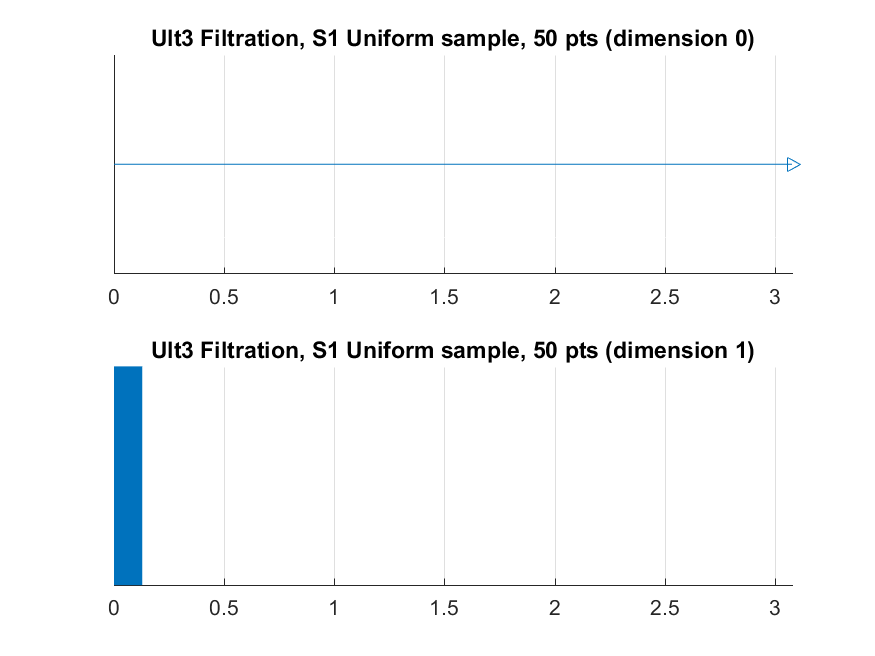
\includegraphics[scale=0.8]{Ult3FiltrationS1Uniformsample50pts.png}
    \caption{The persistence diagram of a equidistributed 50 point sample of $S^1$. }
\end{figure}

We can see how the one-dimensional skeleton of the space is added at time zero, giving a zero-dimensional diagram consisting of just one bar. In the case of the homology of degree 1, all the cycles die at the same time. 

To see what is happening, we can do the next observation. The first radius in which you add simplexes after zero is $\pi/50$. At this time, all triangles that have an edge of length $\pi/50$ are added since we are using geodesic distance. For any triangle that was representing homology before, we can see how a cap made by length $\pi/50$ sided triangles that kills this loop. Then, after this there is no 1-homology.

We also computed $\dgm^{\ult^*_3}_1(S^2).$ For this, we made a FPS \jose{reference needed?} 50 point sample of $S^2$ endowed with the geodesic distance. We obtained the next diagram:

\begin{figure}
	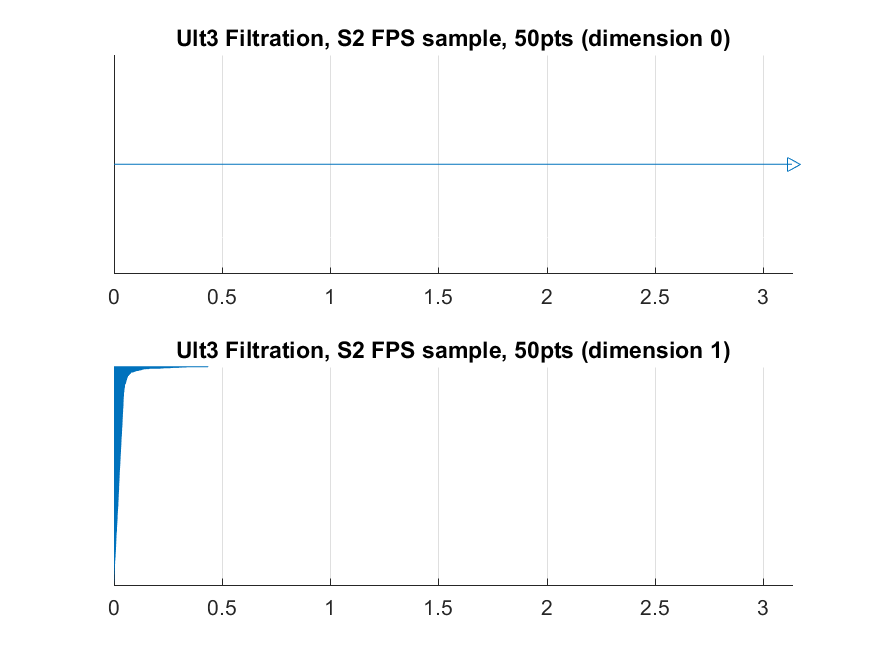
\includegraphics[scale=0.8]{Ult3FiltrationS2FPSsample50pts.png}
    \caption{The persistence diagram of a FPS 50 point sample of $S^2$. }
\end{figure}

We noticed that there is a long bar persisting in this case, that differs from the circle case, in which all bars die at the same time. To understand this, we made a graphic representation of how triangles are added in a simple discretization of the sphere with the geodesic distance. We chose a cube as our discretization. We can describe this as the set:

$$ C= \left\{ \left((-1)^i\frac{1}{\sqrt{2}},(-1)^j\frac{1}{\sqrt{2}}\right) \bigg| i,j=0,1 \right\}\subset S^2 . $$

We endow $C$ with the induced subspace metric $d_C= d_{S^2}|_{c\times C}$, where $d_{S^2}$ is the geodesic distance on $S^2$.

\begin{figure}
	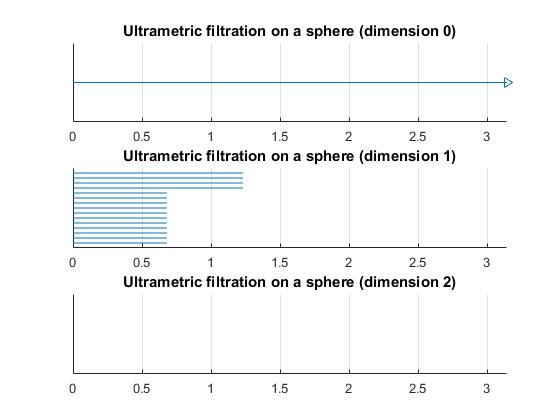
\includegraphics[scale=0.7]{DiagramUlt3Cube.jpg}
    \caption{The persistence diagram of a geodesic cube. }
\end{figure}

\begin{figure}
	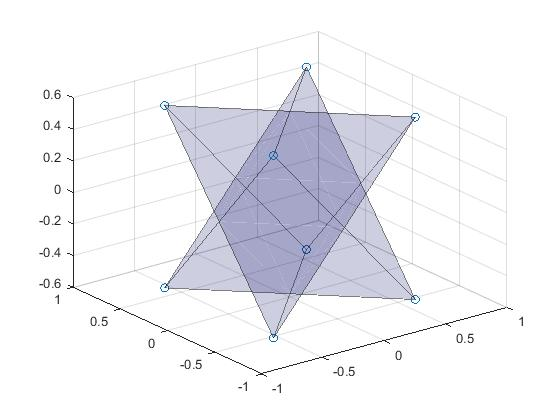
\includegraphics[scale=0.25]{FiltT0cube.jpg}
	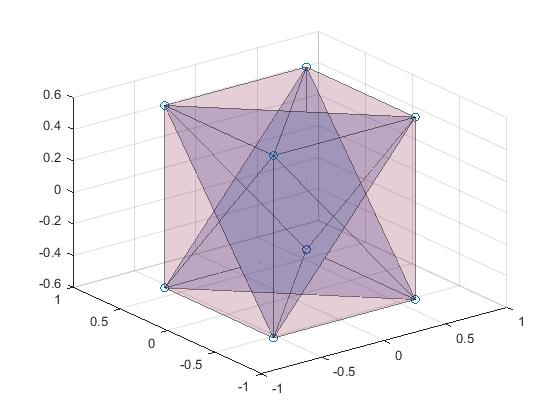
\includegraphics[scale=0.25]{FiltT1cube.jpg}
	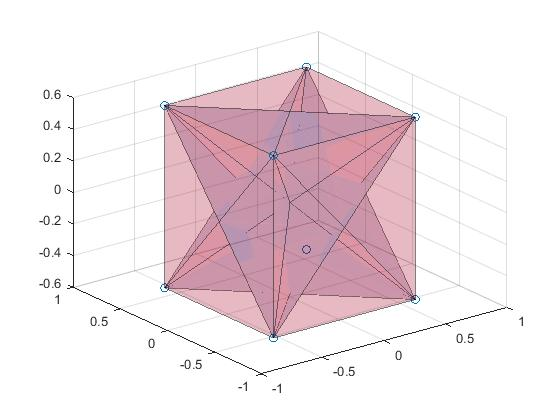
\includegraphics[scale=0.25]{FiltT2cube.jpg}
    \caption{The process of arrival of the 2-dimensional simplexes of the cube on the three relevant times.}
 \end{figure}
 
 \facundo{Jose: por favor describe exactamente cual es el espacio metrico que corresponde al cubo; me confunde lo de 'geodesic cube' etc y por eso parece mejor decir exlicitamente cual es el conjunto subyacente y cual es la metrica/distancia} \jose{ ¿Qué te parece así, Facundo?} \facundo{looks good. Otra cosas relacionadas: (1) los numeros que aparecen abajo deberian ser expresiones exactas en funcion de la geometria (2) enuncia una proposicion con el resultado del los diagramas via ult. EL objectivo es probar esa proposicion eventualmente.} \jose{No me queda 100\% claro qué proposición redactar. En cuanto a las cantidades, tengo que pensar cómo presentarlas. Son longitudes geodésicas que vienen de ángulos no cerrados. Creo que vendría un párrafo explicando cada una. }
 
 In this discretization we can find a similar pattern, with a great majority of bars fating soon and a couple of bars persisting. We can visualize how simplexes are added at each time
 
\begin{itemize}
\item Time 0: two tetrahedron appear, since all faces are equilateral and the ultrametricity of them is zero. 
\item Time 0.6796: we get all triangles that form half faces of the cube. 
\item Time 1.2301: we get all missing triangles.
\end{itemize}


\subsection{The tree functor}

The previously defined ultrametricity filtration detects how close simplices in a space are from being ultrametric. We now can construct a similar filtration based on how close simplices in a space are from being a tree. In the case of ultrametricity, we defined a function $\ult_k:\M\rightarrow \R$ that induced a filtration. This function depends on the fact that we can define a functor $\H:\M\rightarrow \mathcal{U}$ the single-linkage hierarchical clustering. 

In the case of tree spaces, we do not have a unique map that turns a metric space into a tree space. Instead, for each metric space $X$ we will have a family of tree spaces indexed by points in $X$. Given $X\in \M$ and $x^*\in X$, we can define:

\begin{eqnarray*}
	g_{x^*}(x,x')&=& \frac{1}{2}(d_X(x^*,x)+d_X(x^*,x')- d_X(x,x'))\\
    g^\infty_{x^*}(x,x')&= &\max_{x=x_0,...,x_n=x'}\min_{i=1,...,n} g_{x^*}(x_{i-1},x_{i})\\
    t^{x^*}_X(x,x')&=& d_X(x^*,x)+d_X(x^*,x')- 2g^\infty_{x^*}(x,x')
\end{eqnarray*}

We can notice that:

\begin{itemize}
\item the function $t^{x^*}_X: X\times X\rightarrow \R$ is a metric on $X$ and $(X,t^{x^*}_X)$ is a tree space;
\item $t^{x^*}_X(x^*,x)= d_X(x^*,x)$ for all $x\in X$;
\item in general, $t^{x^*}_X(x,x')\leq d_X(x,x')$ for all $x,x'\in X$.
\end{itemize}

Then, for each $X\in\M$ we have a map $\psi:X\rightarrow \mathcal{T}$ given by, 
$$x^*\in X \mapsto (X,t^{x^*}_X)$$


Now, what is the intuition behind this definition? We can think of the space $(X,t^{x^*}_X)$ as a tree that is rooted in $x^*$, and the distance between $x^*$ and any $x\in X$ will be given by the height of the point with respect to $x^*$, that is $d_X(x^*,x)$. 

Given $x,x'\in X$, we can think of $g^{\infty}_{x^*}(x,x')$ as the maximum height in the tree such that $x$ and $x'$ are in the same branch. Then, the distance between $x$ and $x'$ is given by the sum of the heights of $x$ and $x'$ with respect to the point of branch separation. This is given by $t^{x^*}_X$. 

How do we build the tree? The process is the following:
\begin{itemize}
	\item Compute $(g_{x^*}(x,x'))_{x,x'\in X}$.
    \item Order the values on $(g_{x^*}(x,x'))_{x,x'\in X}$ in decreasing order. We can write down as $g_1,...,g_k$. Take $X$ as a set of vertices of a graph with no edges. We will build up a graph over this set of vertices through time, but running from $\infty$ to $0$ instead of the regular order.
    \item For $i=1,...,k$, we add the edge $(x_{(i)},x_{(i)}')$ at time $g_i$ where $(x_{(i)},x_{(i)}')$ is the edge that generated the value $g_i$.
    \item We will have that $g^\infty_{x^*}(x,x')=\inf\{t\geq 0 : x, x' \text{ are disconnected at time }t \}$.
\end{itemize}

\begin{figure}
\centering
\begin{tikzpicture}[scale=0.8,every node/.style={scale=0.8}]
\draw[ultra thick, ->] (4,11) -- (4,-2);

%Points in the tree x^*
\filldraw[black] (9,0) circle (2pt) node[below] {$x^*$};
\filldraw[black] (11+1,10) circle (2pt) node[above] {$x_1$};
\filldraw[black] (11-1,9) circle (2pt) node[above] {$x_2$};
\filldraw[black] (7+1,7.5) circle (2pt) node[above] {$x_3$};
\filldraw[black] (7-1,9) circle (2pt) node[above] {$x_4$};

\draw[gray,dashed] (11+1,10) -- (11+1,0); 
\draw[black] (11+1, 5) node[left] {$d(x^*,x_1)$};
\draw[gray,dashed] (11-1,9) -- (11-1,0); 
\draw[black] (11-1, 4.5) node[left] {$d(x^*,x_2)$};
\draw[gray,dashed] (7-1,9) -- (7-1,0);
\draw[black] (7-1, 4.5) node[left] {$d(x^*,x_4)$};
\draw[gray,dashed] (7+1,7.5) -- (7+1,0); 
\draw[black] (7+1,3.775) node[left] {$d(x^*,x_3)$};
\draw[black,dashed] (4,0) -- (13,0);

\end{tikzpicture}

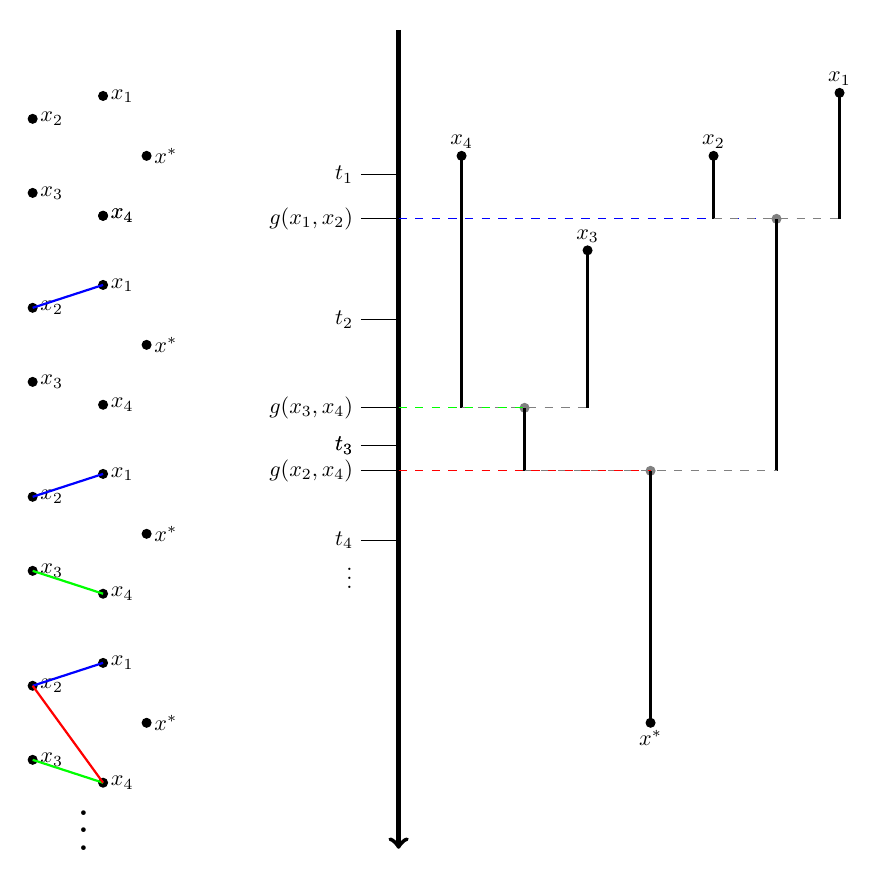
\begin{tikzpicture}[scale=0.8,every node/.style={scale=0.8}]
\draw[ultra thick, ->] (5,11) -- (5,-2);

%Points in the tree x^*
\filldraw[black] (9,0) circle (2pt) node[below] {$x^*$};
\filldraw[black] (11+1,10) circle (2pt) node[above] {$x_1$};
\filldraw[black] (11-1,9) circle (2pt) node[above] {$x_2$};
\filldraw[black] (7+1,7.5) circle (2pt) node[above] {$x_3$};
\filldraw[black] (7-1,9) circle (2pt) node[above] {$x_4$};

%\pause
% First penthagon
\filldraw[black] (1,9) circle (2pt) node[anchor=west] {$x^*$};
\filldraw[black] (0.309,9.9511) circle (2pt) node[anchor=west] {$x_1$};
\filldraw[black] (-0.809,9.5878) circle (2pt) node[anchor=west] {$x_2$};
\filldraw[black] (-0.809,9-.5878) circle (2pt) node[anchor=west] {$x_3$};
\filldraw[black] (0.309,9-0.9511) circle (2pt) node[anchor=west] {$x_4$};
\filldraw[black] (0.309,9-0.9511) circle (2pt) node[anchor=west] {$x_4$};
% Time highlight
\draw[shift={(5-0.3,8.7)},color=black] (-0.3,0) -- (0.3,0) ;
\draw[black] (5-0.6,8.7) node[left] {$t_1$};


%\pause
%Second Penthagon
\filldraw[black] (1,6) circle (2pt) node[anchor=west] {$x^*$};
\filldraw[black] (0.309,6.9511) circle (2pt) node[anchor=west] {$x_1$};
\filldraw[black] (-0.809,6.5878) circle (2pt) node[anchor=west] {$x_2$};
\filldraw[black] (-0.809,6-.5878) circle (2pt) node[anchor=west] {$x_3$};
\filldraw[black] (0.309,6-0.9511) circle (2pt) node[anchor=west] {$x_4$};
\draw[blue,thick] (0.309,6.9511) -- (-0.809,6.5878);
% Distinction line G1
\draw[shift={(5-0.3,8)},color=black] (-0.3,0) -- (0.3,0) ;
\draw[black] (5-0.6,8) node[left] {$g(x_1,x_2)$};
\filldraw[gray] (11,8) circle (2pt) ;
\draw[thick] (11+1,8) -- (11+1,10);
\draw[thick] (11-1,8) -- (11-1,9);
\draw[dashed,blue] (5,8) -- (11,8);
\draw[dashed,gray] (11-1,8) -- (11+1,8);
% Time highlight
\draw[shift={(5-0.3,6.4)},color=black] (-0.3,0) -- (0.3,0) ;
\draw[black] (5-0.6,6.4) node[left] {$t_2$};

%\pause
%Third penthagon
\filldraw[black] (1,3) circle (2pt) node[anchor=west] {$x^*$};
\filldraw[black] (0.309,3.9511) circle (2pt) node[anchor=west] {$x_1$};
\filldraw[black] (-0.809,3.5878) circle (2pt) node[anchor=west] {$x_2$};
\filldraw[black] (-0.809,3-.5878) circle (2pt) node[anchor=west] {$x_3$};
\filldraw[black] (0.309,3-0.9511) circle (2pt) node[anchor=west] {$x_4$};
\draw[blue,thick] (0.309,3.9511) -- (-0.809,3.5878);
\draw[green,thick] (-0.809,3-.5878) -- (0.309,3-0.9511);
% Distinction line G2
\draw[shift={(5-0.3,5)},color=black] (-0.3,0) -- (0.3,0) ;
\draw[black] (5-0.6,5) node[left] {$g(x_3,x_4)$};
\filldraw[gray] (7,5) circle (2pt)  ;
\draw[thick] (7-1,5) -- (7-1,9);
\draw[thick] (7+1,5) -- (7+1,7.5);
\draw[dashed,green] (5,5) -- (7,5);
\draw[dashed,gray] (7-1,5) -- (7+1,5);
% Time highlight
\draw[shift={(5-0.3,4.4)},color=black] (-0.3,0) -- (0.3,0) ;
\draw[black] (5-0.6,4.4) node[left] {$t_3$};

%\pause
% Forth pentagon
\filldraw[black] (1,0) circle (2pt) node[anchor=west] {$x^*$};
\filldraw[black] (0.309,.9511) circle (2pt) node[anchor=west] {$x_1$};
\filldraw[black] (-0.809,.5878) circle (2pt) node[anchor=west] {$x_2$};
\filldraw[black] (-0.809,-.5878) circle (2pt) node[anchor=west] {$x_3$};
\filldraw[black] (0.309,-0.9511) circle (2pt) node[anchor=west] {$x_4$};
\draw[blue,thick] (0.309,.9511) -- (-0.809,.5878);
\draw[green,thick] (-0.809,-.5878) -- (0.309,-0.9511);
\draw[red,thick] (-0.809,.5878) -- (0.309,-0.9511);
% Distinction line G3
\draw[shift={(5-0.3,4)},color=black] (-0.3,0) -- (0.3,0) ;
\draw[black] (5-0.6,4) node[left] {$g(x_2,x_4)$};
\filldraw[gray] (9,4) circle (2pt)  ;
\draw[thick] (7,4) -- (7,5);
\draw[thick] (11,4) -- (11,8);
\draw[dashed,red] (5,4) -- (9,4);
\draw[dashed,gray] (9-2,4) -- (9+2,4);
% Time highlight
\draw[shift={(5-0.3,4.4)},color=black] (-0.3,0) -- (0.3,0) ;
\draw[black] (5-0.6,4.4) node[left] {$t_3$};





%\pause
%Final step
\draw[thick] (9,0) -- (9,4);
% Time Highlight
\draw[shift={(5-0.3,2.9)},color=black] (-0.3,0) -- (0.3,0) ;
\draw[black] (5-0.6,2.9) node[left] {$t_4$};

\draw[dashed,green] (5,5) -- (7,5);
\draw[dashed,red] (5,4) -- (9,4);
\draw[black] (0, -1.5) node[scale=2,thick] {$\vdots$};
\draw[,black] (5-0.6,2.4) node[left,thick] {$\vdots$};

\end{tikzpicture}
\caption{A representation of the graph-building process through the $G-$filtration and the resulting tree space. (Above) We first place all points of the space at height $d_X(x^*,x_i)$ from $x^*$. (Below) Each graph on the left represents the graph at time $t_i$ for $i\in \{1,2,3,4\}$. The distances between points in the tree space are given by the sum of vertical distance between two points in this tree. }
\end{figure}


We can notice that this process generates a graph that changes over time that depends on the metric structure of $X$. It is possible to define a filtration from the graph structure. An important thing to observe is that this is not a growing structure: it is decreasing over time if we go from $0$ to $\infty$ in the positive direction. 

\defn{ Let $(X,d_X)$ be a metric space. A reverse filtration on $X$ is a function $F:\pow(X)\rightarrow \R$ such that for all $\tau\subset \sigma\subset X$, $F(\tau)\geq F(\sigma)$. The complex that it induces can be expressed as:
\begin{eqnarray}
	X_{t}&=& \{\sigma \subset X : F(\sigma)\geq t\}.
\end{eqnarray}
}

We can define a formal filtration over the graph that we generated. It will be the clique complex \jose{better flag complex? Reference?} generated by the filtration graph.

\defn{Let $X\in\M$ and $x^*\in X$. We define the $G-$filtration on $X$ based on $x^*$ to be $G^{x^*}_{X}: \pow(X)\rightarrow \R$ given by:

$$G^{x^*}_X(\sigma)= \min_{x,x'\in \iota_X(\sigma)} g_{x^*}(x,x'). $$

This induces a reversed basepoint filtration functor $G:\M \rightarrow \pow(\F)$ given by:
$$G_X(x^*)= G^{x^*}_X, \hspace{1cm} \forall \, X\in \M, \, x^*\in X.$$
}\\

Thinking in terms of a stability theorem, we would like to have a way of comparing this filtration. We can adapt the definition we already have for filtered spaces to come up with a definition of distance between reversed filtrations.

\defn{If $X,Y\in \M$ and $F_X,F_Y$ are reversed filtrations on $X$ and $Y$ respectively, we define the reversed filtration distance between $F_X$ and $F_Y$ to be,
$$ d_{\F}(F_X,F_Y)= \inf_{Z, \phi_X,\phi_Y}\max_{\sigma \subset Z} |F_X(\phi_X(\sigma))-F_Y(\phi_Y(\sigma))|.$$}

We can define the function $\nu_3: \pow(\R^{3\times 3}) \rightarrow \R$:

$$\nu_3(A) =\frac{1}{2}\min_{a\in A} (a_{12}+a_{13}-a_{23}).$$

It is possible to prove that $\nu_3$ is a $3-$stable valuation. Since $G_X(x^*)(\sigma)= \nu_3(\cset(x^*,\iota_X(\sigma)))$, the $G-$filtration is a $2$-local reversed basepoint filtration functor Then, the following theorem follows:

\begin{thm}\label{thm:stabtree}
Let $X,Y\in \M$. Then, 
$$ 6\dgh(X,Y)\geq \inf_{R}\max_{(x^*,y^*)\in R}d_{\F}((X,G_X(x^*)), (Y,G_Y(y^*)) ).$$
\end{thm}

To visualize how it behaves in particular spaces, we programmed a MATLAB code using the javaplex package. We can compute the diagrams of discretizations of the sphere, the 2-torus and the 3-torus to see the behavior of the $G-$filtration on this spaces choosing an arbitrary point. Since this spaces are symmetric, the choice of points was arbitrary. 

First, we can notice how $S^2$ does not have 1-dimensional homology. It is interesting how the diagrams of the 2-torus and the 3-torus have considerable 1-homology; mainly that the torus has two long bars. It seems that this filtration is capturing important topological features of spaces. 


\begin{figure}
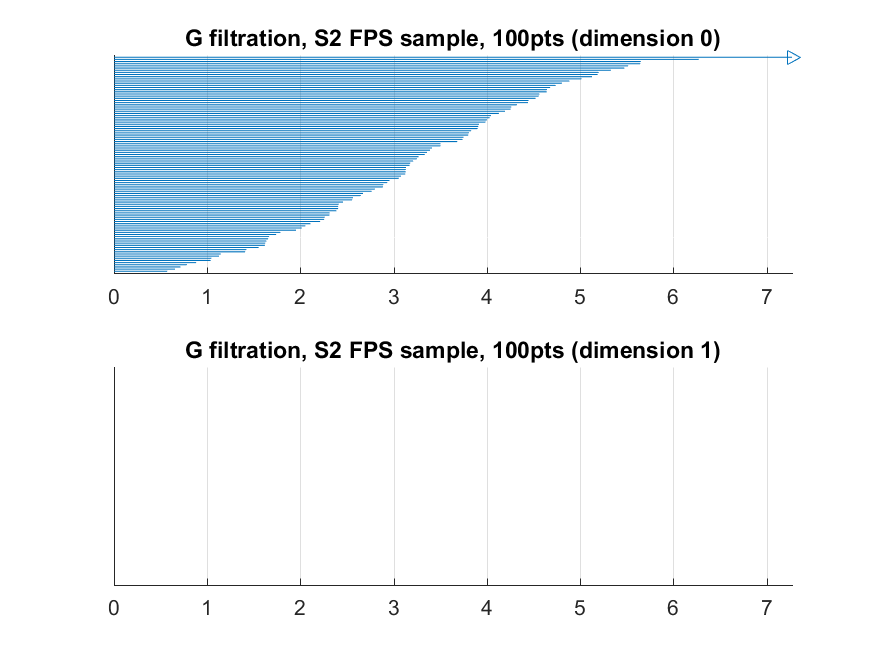
\includegraphics[scale= 0.7]{GFiltS2FPS100pts.png}
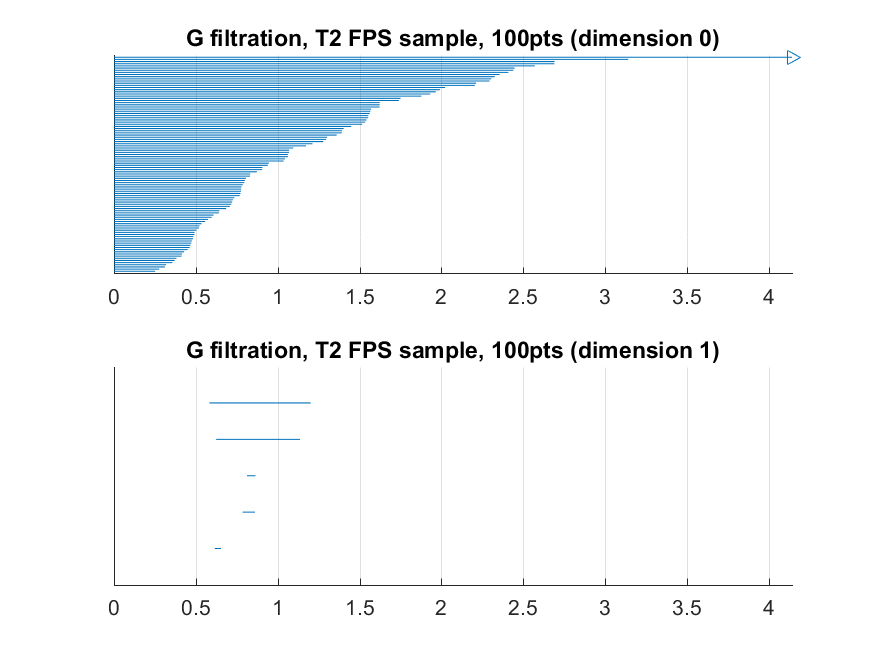
\includegraphics[scale= 0.7]{GFiltT2FPS100pts.png}
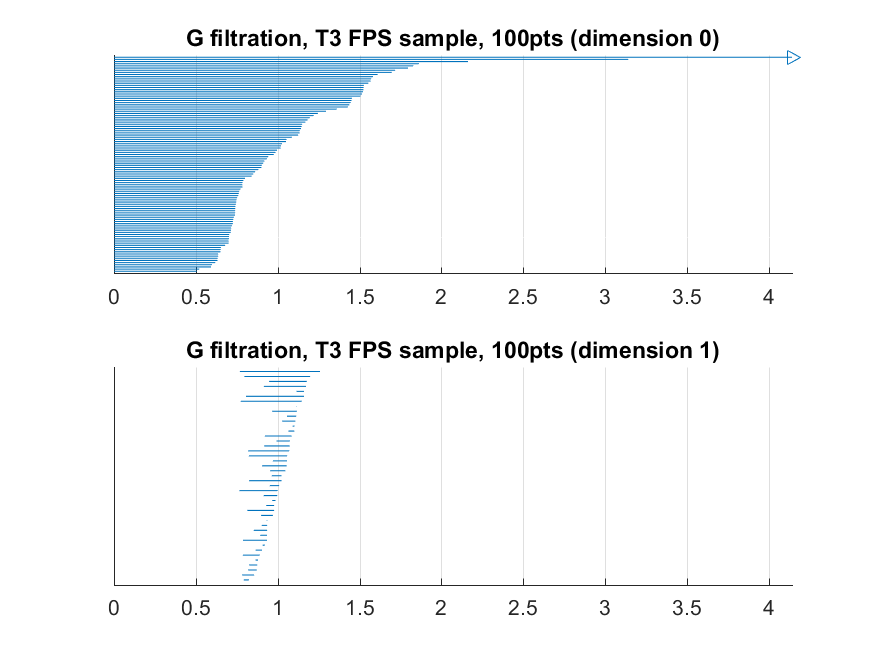
\includegraphics[scale= 0.7]{GFiltT3FPS100pts.png}
\caption{A presentation of the $G-$filtration diagrams on a FPS 100 point sample of (above) $S^2$ with geodesic distance, (middle) $T^2$ with the $\ell_{\infty}$ product metric, and (bellow) $T^3$ with the $\ell_{\infty}$ product metric. We plot time in reverse order, meaning that in the $x-$axis, $t\rightarrow \diam(X)-t$.}
\end{figure}


\section{Pushforward constructions}
\facundo{to develop...}

\begin{thebibliography}{9}
\bibitem{dgh-props} Facundo Memoli. Some Properties of Gromov-Hausdorff Distances. Discrete Comput. Geom. 48, 2 (September 2012), 416-440. 

\bibitem{tripods}  Facundo Memoli. "A Distance Between Filtered Spaces Via Tripods." arXiv preprint arXiv:1704.03965 (2017).

\bibitem{clustering} Gunnar Carlsson and Facundo Memoli. Characterization, Stability and Convergence of Hierarchical
Clustering Methods. Journal of Machine Learning Research. 11 (2010), 1425-1470.

\end{thebibliography}
\end{document}